\section*{Instrucciones:}

\begin{itemize}
    \item Entrega en un pdf las respuestas de los ejercicios que no requieran implementarse y añade una breve descripción de los programas que entregas (sus nombres y qué hacen).
    
    \item Los programas deben ir un zip. Debes realizar un programa en cada ejercicio que indique “Implemetar”.

    \item Recuerda que debes utilizar Java 21 LTS.

    \item \textbf{Si no compila utilizando Java 21LTS o si no se entrega la breve descripción de los
    programas se penalizará.}
\end{itemize}

\textbf{Tiempo de elaboración:} $\approx$ 1.5 hrs

\textbf{Total de puntos:} 100

\section*{Ejercicios:}

\begin{enumerate}
    \item Lee lo siguiente \href{https://www.evanjones.ca/software/threading-linus-msg.html}{https://www.evanjones.ca/software/threading-linus-msg.html} y comparte en máximo 4 líneas de computadora a que se refiere Linus Torvalds con un contexto de ejecución y cómo se relaciona con la definición en la sección 1 de esta práctica.

    Recordando la distinción conceptual introductoria hecha para práctica entre procesos e hilos, bajo los ojos de Linus Trovalds en la parte práctica no importa tanto estas distinciones y es mejor mirarlo desde la visión del ''contexto de ejecución'', un ejemplo es Linux, donde son vistas como tareas y bajo estas reglas se diseñan las tareas en el Kernel.

    \hfill
    
    \item  ¿Cuántos hilos tiene disponibles tu computadora?
    
    \textit{Ejecuta Runtime.getRuntime().availableProcessors(), si son más de uno en el equipo escriban el de cada uno.}

    Con base a la ejecución de Runtime.getRuntime().availableProcessors() para cada computadora:

    \begin{figure}[h]
        \centering
        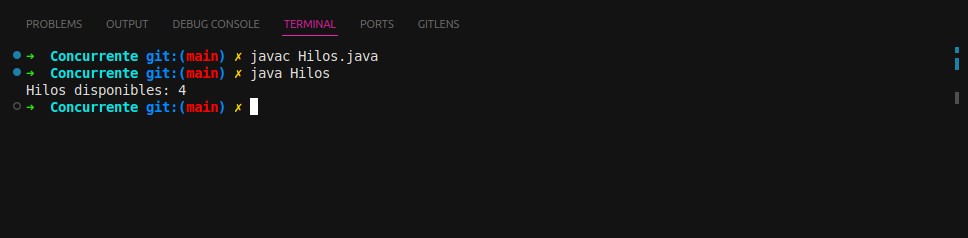
\includegraphics[width=0.8\textwidth]{resources/Ej2.png}
        \caption{Computadora de Fernanda: 4}
    \end{figure}
    
    Computadora de Huriel: 12

    Computadora de Hugo: 12

    \hfill
    
    \item Revisa el programa Determinante concurrente y responde ¿Cuánto tiempo tarda en ejecutarse?

    \begin{figure}[h]
        \centering
        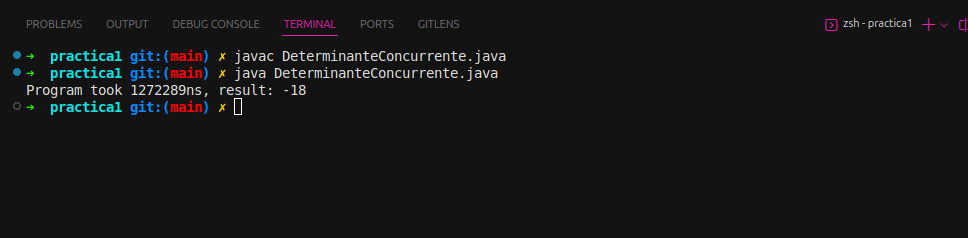
\includegraphics[width=0.8\textwidth]{resources/Ej3.png}
    \end{figure}

    \hfill    

    \item El programa Determinante concurrente está implementado extendiendo la clase Thread. Implementa el programa utilizando la interfaz Runnable.
    El programa DeterminanteConcurrenteRunnable.java usa runnable lo cual es más flexible y evitamos la herencia de Thread, hacemos los mismos cálculos para obtener el determinante de una matriz y mostramos el cálculo de toda la determinante al final.

    \begin{figure}[h]
        \centering
        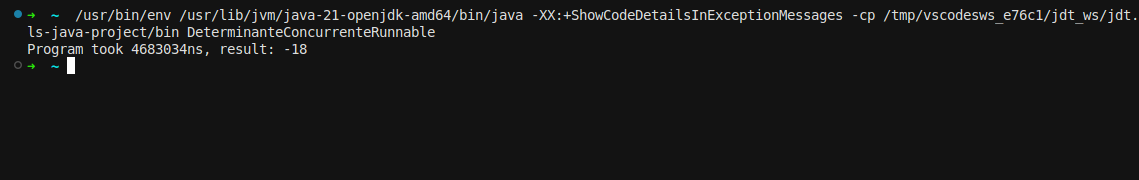
\includegraphics[width=0.8\textwidth]{resources/Ej4.png}
    \end{figure}

    \hfill
    
    \item Implementa el programa Determinante concurrente de forma secuencial.

    El programa DCsecuencial.java calcula el determinante de una matriz 3x3 de manera secuencial utilizando la regla de Sarrus, esta regla establece un método          directo para calcular el determinante de matrices 3x3 sumando y restando productos de elementos específicos de la matriz. El programa define una matriz de          prueba y luego ejecuta una función que aplica la regla de Sarrus sobre ella, además, se mide el tiempo de ejecución utilizando System.nanoTime(), al final, 
      el programa imprime el tiempo de ejecución en nanosegundos y el valor calculado del determinante, este enfoque no involucra concurrencia, ya que todo el 
      cálculo se realiza de forma secuencial en un solo hilo.

    \hfill
    
    \item Implementa del programa Determinante concurrente para dos hilos (en vez de seis).

    El programa DCdosHilos.java calcula el determinante de una matriz 3x3 de manera concurrente utilizando dos hilos, la matriz de prueba se divide en dos partes      para que cada hilo se encargue de calcular una sección del determinante utilizando la regla de Sarrus, el primer hilo se encarga de calcular los tres términos     positivos de la regla, mientras que el segundo hilo calcula los tres términos negativos. Ambos hilos se inician de forma simultánea y luego se espera a que        ambos terminen utilizando join(). Al finalizar, los resultados parciales calculados por cada hilo se suman para obtener el determinante total, el programa         también mide el tiempo de ejecución en nanosegundos y lo imprime junto con el resultado calculado, esta implementación busca mejorar el tiempo de cálculo          dividiendo el trabajo en dos hilos, a diferencia del enfoque secuencial.

    \hfill

    \item Compara las 3 implementaciones: el programa Determinante concurrente para dos hilos, para seis hilos y el programa secuencial. Responde: ¿A qué se debe el orden en el que se ordenan los tiempos de ejecución de cada programa?

    \begin{itemize}
        \item \textbf{Secuencial:} 1500 ns
        \item \textbf{Dos hilos:} 408600 ns
        \item \textbf{Seis hilos:} 680100 ns
    \end{itemize}

    \begin{itemize}
        \item \textbf{Secuencial (1500 ns):} El tiempo de ejecución del programa secuencial es el más bajo porque realiza todos los cálculos en un solo hilo, sin            ningún tipo de paralelización ni sobrecarga de gestión de hilos, en este caso, el programa es sencillo y directo, no es necesario crear, gestionar o                sincronizar hilos, entonces, gracias a la pequeña cantidad de operaciones, el tiempo es mínimo.
    
        \item \textbf{Dos hilos (408600 ns):} El uso de dos hilos mejora la paralelización, pero no necesariamente mejora el tiempo de ejecución, en este caso, la           creación de los hilos y la sincronización entre ellos da paso a una sobrecarga que aumenta el tiempo de ejecución en comparación con la implementación              secuencial, aunque se distribuye el cálculo de los términos del determinante entre dos hilos, la sobrecarga asociada con la creación de los hilos y la              espera de su finalización (sincronización) supera las ventajas de la paralelización, por lo que, se tiene un mayor tiempo de ejecución.
    
        \item \textbf{Seis hilos (680100 ns):} A pesar de que más hilos teóricamente podrían dividir la carga de trabajo, en este caso, la implementación con seis           hilos tiene el mayor tiempo de ejecución por la gran sobrecarga en la gestión de hilos. Con seis hilos, el sistema debe crear, gestionar y sincronizar un           mayor número de hilos, como consecuencia, tarda más y rinde menos. Este tipo de paralelización se vuelve ineficiente cuando el problema es demasiado                pequeño, ya que la sobrecarga de los hilos supera el tiempo de cálculo real.
\end{itemize}

Tomando en cuenta los argumentos anteriores, decimos que a pesar de que la paralelización con más hilos teóricamente podría mejorar el rendimiento, la sobrecarga asociada con la creación y sincronización de hilos es mucho más costosa en términos de tiempo cuando se trabaja con tareas pequeñas y simples, en este caso, el cálculo del determinante de una matriz 3x3. Por lo tanto, el programa secuencial es el más eficiente en este caso, seguido por el uso de dos hilos, y finalmente el de seis hilos, que presenta la mayor sobrecarga.


    \hfill    
    
    \item Si utilizas la Ley de Amdahl entre el programa Determinante concurrente para dos hilos y el programa secuencial. ¿El resultado es mayor o menor a 1? ¿Por qué?

    Recordando nuestra fórmula de la ley de Amdahl:

    \[ S = \frac{1}{1-p + \frac{p}{n}}\]

    Interpretando esta misma, recordemos que nuestro resultado va a ser dependiente a la cantidad de trabajo paralelizable y a la cantidad de hilos a los cuales les podamos distribuir trabajo paralelizable, sabemos que en ambos programas mencionados en la descripción del ejercicio, la cantidad de hilos es 2 ($n=2$) y 1 ($n=1$) respectivamente.

    Vamos a calcular la Ley de Amdahl en base a nuestros resultados, donde obtuvimos que DeterminanteConcurrente tardó 728,270 ns y el secuencial sólo 6,961 ns, con lo cuál
    podemos ver el speedup de la Ley de Amdahl:

    \[S = \frac{T_s}{T_p}=\frac{6961}{728270}=0.0095582\]

    Por lo que el speedu es menor a 1, lo cual significa que la versión concurrente es mucho peor o es más lenta que la secuencial, el por qué de esto es porque tenemos en el concurrente la creación de 6 hilos, por lo que esto es un proceso el cual a la computadora le lleva su tiempo hacerlo. Ahora, si vemos el secuencial, este tiene unas operaciones sobre una matriz de 3x3 que no representan gran costo computacional, en este caso entonces la creación de hilos sí es significativa para nuestro programa.
    Al final, también tenemos la gestión del join, el cual también representa un costo que a este nivel sí es significativo.
    Con esto, podemos concluir que la concurrencia es significativa cuando se tiene una gran cantidad de datos a procesar y operaciones de gran tamaño, en este caso al el tamaño
    de la matriz es muy pequeña, la gestión de los hilos, creación, inicio, sincronización, sí es significativa.
    Podemos notar que en sí el resultado que buscamos obtener es muy rápido de obtener.

    Resultado de cada proceso 

    \begin{figure}[h]
        \centering
        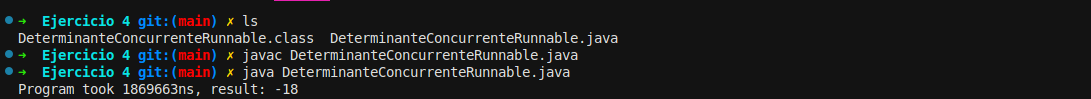
\includegraphics[width=0.8\textwidth]{resources/Ej8_4.png}
    \end{figure}

    \begin{figure}[h]
        \centering
        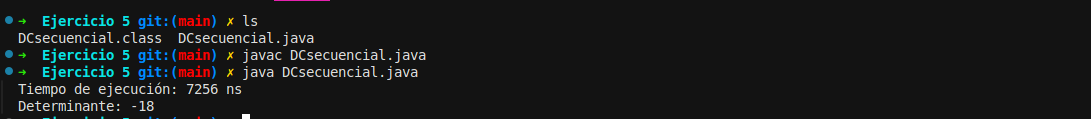
\includegraphics[width=0.8\textwidth]{resources/Ej8_5.png}
    \end{figure}

    \hfill    
    
    \item Describe con tus propias palabras en máximo dos líneas para qué sirve el método join(). Si no utilizas el método join() en Determinante Concurrente, ¿sigue funcionando?

    La función principal del método join() es permitir que los hilos terminen de ejecutar sus tareas asignadas sin el riesgo de que el main deje de operar y así poder obtener el producto de nuestras matrices de forma segura.
    
    En caso de que deseemos realizar un programa análogo a Determinante Concurrente sin un método de funcionamiento similar a nuestro método join(), tenemos el problema de que al estar trabajando con operaciones ejecutadas en modo concurrente, no haya un lapso de espera necesario para calcular todas las operaciones necesarias para otorgar el producto de matrices correcto, por lo cual siempre se necesitará de alguna ''espera'' para que todos los hilos terminen antes de concluir nuestra ejecución.

    \hfill
    
\end{enumerate}
